\documentclass[a4paper]{article}

%% Useful packages
\usepackage{amsmath}
\usepackage{graphicx}
\usepackage[colorinlistoftodos]{todonotes}
\usepackage[colorlinks=true, allcolors=black]{hyperref}
\usepackage[fontsize=11pt]{scrextend}
\usepackage{titlesec}
 \usepackage[section]{placeins}

\setlength\parindent{0pt}
\titleformat*{\section}{\Large\bfseries}
\titleformat*{\subsection}{\Large\bfseries}

\title{RASD - Requirements And Specifications Document}

\begin{document}

\begin{titlepage}
\begin{figure}
\centering

\includegraphics[width=0.2\textwidth]{polimi.jpg}
\par
\LARGE Politecnico di Milano
\end{figure}


\maketitle
\textbf{Version 1.1}
\newline

\raggedright
Authors:
\begin{itemize}
	\item Domenico FAVARO (Mat. 837995)
        	\item Matheus FIM (Mat. 876069)
	\item Caio ZULIANI (Mat. 877266)	
\end{itemize}
\raggedleft
Prof. Elisabetta DI NITTO
\thispagestyle{empty}
\end{titlepage}

\tableofcontents
\newpage
 
\section{Introduction}
\subsection{Problem Definition - PowerEnJoy}
The requested System denoted PowerEnJoy, is a car-sharing service that  exclusively employs electric Cars. 
\newline\newline
As a car-sharing service it should allow the use of a Car via Reservation, taking it and bringing it back to determined parking areas and paying for the use made.
\newline\newline
The System should allow Users to register so it can authorize them to use the car-sharing services, and allow them to reserve an available Car near their location or on a given address, so they can use it for a ride. 
\newline\newline
The Users will provide their credentials and payment info so all the transactions for the service use are made automatically by the System.
\newline\newline
The System should incentivize Virtuous Behaviors of the Users by providing extra discounts, or fees in case of misconduct, on the current ride. These Virtuous Behavior rules will compensate service expenses for the Cars, specially re-charging costs.
\newline\newline
The System should provide these functionalities based on a mobile and web application that can be used by Registered Users to use the PowerEnJoy services. The System should interface as well with the Car so it can obtain important information from it, like location and battery use, and so it can control its locking or unlocking for the use.
\newline\newline
For any issue that the User may find using the service or also for any incident a User may cause to the service, we've designed a Customer Relationship Manager (CRM) who'll be allowed to check the status of the Cars and Users, and be able to solve any inconvenient presented during the use of the service. 

\newpage
\subsection{Goals}
\textbf{User:}
\begin{description}
\item [G.1)]First-Time Users must be able to register to the System creating an Account. 
\item [G.2)]Registered Users must be able to login to their Account at any time they want.
\item [G.3)]Users can save his/hers credentials in the System.
\item [G.4)]A Registered User will be able to make a Reservation of any available Car near his/her current location or from an address that she/he can specify.
\item [G.5)]Users that had made a Reservation must be able to notify the System when they are nearby the Reserved Car so the System can unlock it.
\item [G.6)]A User that has made a Reservation must be able to cancel it before 1 hour starting from the time when the Reservation was made.
\item [G.7)]In case an User hasn't started using the Reserved Car at 45 minutes after the Reservation was made, he/she will be notified that either if the Reservation is not canceled or the Car is not used in 15 minutes, the Reservation will be automatically canceled and a 1 Euro fee will be charged to her/his Account.
\item [G.8)]When Users that start using their Reserved Car, they must be able to see their current expenses on the service through a System screen inside the Car.
\item [G.9)]The User must be able to know where the safe parking areas are nearby his/her current location or any address that she/he can specify.
\item [G.10)]Users must be able to finish their use of the Car when leaving it in a Safe Parking Area and exiting the car. The User will then be charged for the use of the service. The used Car will be locked and freed for Users to be reserved.
\item [G.11)]The User will always be notified when any Transaction is made on his Account.
\item [G.12)]Notify the Users that are currently using a Car of any available discounts on their ride if they abide by the 'Virtuous Behaviour' rules and of the extra fee in case of not respecting the facilitation of the re-charging of the Car on site. These extra discounts/charges will be applied on the Total fee at the end of the ride. These rules are:
\begin{description}
\item [G.12.1)]Apply a 10\% discount if the User takes at least 2 other passenger into the car.
\item [G.12.2)]Apply a 20\% discount if the User leaves the Car with the battery at least half-full.
\item [G.12.3)]Apply a 30\% discount if the User leaves and plugs the Car in a Re-Charging Station.
\item [G.12.4)]Apply a 30\% extra fee if the User leaves the Car at more than 3KM from the nearest Re-Charging Station.
\item [G.12.5)]Apply a 30\% extra fee if the User leaves the Car with the battery less than 20\% full.
\end{description}
\item [G.13)]Users can activate the Money Saving option on their Account to be notified of any nearby Re-Charging station on their arrival destination. Leaving the car at the end of the ride t this station and plugging it will register as a 'Virtuous Behavior' and will apply and extra discount when charging the User.
\item [G.14)]Users must have the option to contact a CRM at any moment, the System must provide a Customer Service area that offers a Chat feature within the App or a phone number.
\end{description}
\textbf{CRM:}
\begin{description}
\item [G.15)]CRM must be able to log in into the System with an Account and see a list of all the Cars available, reserved, in use or unavailable.
\item [G.16)]CRM has to be able to receive User Reports via chat or outside the app via phone call and be able to register it to the System.
\item [G.17)]CRM upon request form an User or any major cause can Reserve or cancel any active Reservation.
\item [G.18)]CRM must be able to change the Status of a Car given a User Report and tag it, in case it's unavailable, if it's due to Re-Charge, Fix, or Removal.
\item [G.19)]Upon the completion of an User Report CRM must be able to apply extra fees or refund the payment to any User in case the situation demands it.
\end {description}

\newpage
\subsection{Glossary}
\begin{itemize}
\item \textbf{First-Time User:} A User that has not created an Account and thus has not yet been registered by the System. Can have a client version of the application, but he/she can't use the service until Registered.
\item \textbf{Registered User/Users:} A User that has provided valid credentials and payment information to create an Account in the System.
\item \textbf{Account:} Allows the Registered User or the CRM to authenticate to the System and access the car-sharing service.
\item \textbf{Car:} An electric motored vehicle registered to the PowerEnJoy car-sharing service and thus interfaced to the System. It can be available for reservation, reserved, ready to use, on use and unavailable.
\item \textbf{Reservation:} Option for the User to denote their future use of an available Car. Once activated it marks the Car as Reserved and is active until the User starts the use of the Car or until 1 hour after its activation, at which point it's cancelled and an user fee is applied.
\item \textbf{Ride:} The actual use of the Car by the User. It starts when the User ignites the Car engine for the first time and it ends when the car is parked in a safe area and the User exits the Car.
\item \textbf{Safe Parking Area:} Pre-defined areas by the System where a Car can be left by the User to be able to finish their ride.
\item \textbf{Fee:} Amount of money that is due by the User for any of the System services or for any User misbehavior.
\item \textbf{Transaction:} Any exchange of money made by the System on the User Account, every fee payment is a transaction.
\item \textbf{Re-Charging Station:} Special stations where the Cars can be left and plugged in to have their battery re-charged. They count as Safe Parking Areas.
\item \textbf{Virtuous Behavior Rule:} Any of the incentive rules that provide the user with a discount on their current ride if they follow it.
\item \textbf{Status of the Car:} It is the name of a check list made by the car's System at the end of each ride. This check list consists in the status of battery, the number of passengers on the car, if the car is plugged on a recharge station and their localization.
\item \textbf{CRM:} or Customer Relationship Manager will be an employee able to Log in to the System with special privileges to update reservation, car status, transactions, etc. in order fix any eventuality an User may find during his/her use of the service.
\item \textbf{User Report:} A User that has contacted a CRM or a major cause that would create a problem in the System will register into the system as a User Report, made by a CRM. This Report can describe for example an incident, a defect during the ride or a Car that has been fined, and will include if necessary a fine or a refund to the User depending on the case.
\item \textbf{App:}  Smartphone application that does the interface between the User and the System.
\item \textbf{Main Page:} A page within the app where a map is showed centered in the users position.
\end{itemize}

\subsection{Domain Assumptions}
As not all aspects of the given world are considered in the problem definition, the following domain assumptions will be made so they hold for the entirety of the project.
\begin{itemize}
\item Once Users have registered with valid payment information, all payments made with their Account will be valid and arrive successfully.
\item GPS locations on Users and Cars will always be valid.
\item Available Cars will be always in good working conditions.
\item Users that have made a Reservation will always be able to follow its status until the end of the ride, meaning that the screen on the Car will stay functional or by defect their use of the mobile app will not be interrupted by missing connection or empty battery on their mobile device.
\item Once a Car is Picked Up and Unlocked we assume the Users will follow to start its engine and proceed with the Ride. 
\item The Cars will be equipped with weight sensors on each seat so it can detect how many passengers they are on a ride as well as being able to issue seat belt warnings.
\item All Cars on the service will be at least 5 seat Cars so the option to take 2 passengers or more is always available.
\item All Available Cars will have at least 20\% battery left, all Cars not available because of low battery will be alerted by a CRM and will be moved by the service personnel to a Re-Charge station by the end of the day. 
\item Reservations take immediate effect so no conflict of concurrency can happen for a Car, it cannot belong to more than one Reservation at once.
\item CRM will be employees of the service that will be registered directly into the database, the System does not need to allow the option for them to Register. 
\item CRM will be working in an office able to login to the web application of the System, with an office phone available and we assume there will be at least one available at every hour the Service is working. 
\end{itemize}

\subsection{Constraints}
As the problem description has not explained every aspect of the System in detail, we'll impose the following constraints that'll ensure the consistency and good functioning of our System.
\begin{itemize} 
\item Users will be able to have at most one active Reservation at a time.
\item Cars can have at most one Reservation active at a time and only one active Ride that originates from that Reservation.
\item Once a Car is Picked Up a Ride is created by the Reservation and the base fee is set for that Ride, even if the User does not move the Car.
\item If a Car is left parked Unlocked in an active Ride for any reason (not confirming the end of the Ride) after one hour the System should Lock it and end the current Ride.
\item Fee Calculation will have a base Fee, that is applied as soon as the Ride is created and will have a fixed fee by minute of use from the moment the User ignites the Engine. When the Ride is finished, the discounts (or extra fees) will deduce from these subtotal to get the Total Fee of the Ride.
\item To avoid misusage of the Reservations and cancelation a CRM will be notified when an User has made and canceled 3 reservations in a row and will be able to block the User Account for an ammount of time that will deny him from any Reservation during that time.

\end{itemize}

\subsection{Stakeholders}
Our Main Stakeholder is the PowerEnJoy Car-Sharing Service, owned by Prof. DiNitto, that wants a management System for the main functionalities of its service.

\subsection{Reference Documents}
\begin{itemize}
\item Specification Document: Assignments AA 2016-2017.pdf
\item IEEE Std 830-1998 IEEE Recommended Practice for Software Requirements Specifications (IEEEXplore-SRS-template.pdf)
\item Scenario-based Requirements Engineering (ScenarioPaper.pdf)
\item Example Documents:
\begin{itemize}
\item[-] RASD sample from Oct. 20 lecture.pdf - myTaxiService
\item[-] RASD esempio.pdf - Management Project Homework
\end{itemize}
\end{itemize}

\newpage
\section{Proposed System}
\label{sec:propSystem}
Our Proposed System consist in a 3-tier Client-Server Architecture, with web clients for Users and CRM, mobile App clients for Users and the Car interface that will be implemented as a Client as it's external to our Server System. The Server side will consist on a Java EE Server that will implement a Web Tier for Web Clients and a Business Tier that'll communicate directly to the App Clients. The Server will then connect to the Company's Database that'll be located in our EIS Tier.
\begin{figure}[h]
\centering
\vspace*{\fill}
\noindent\makebox[\textwidth]{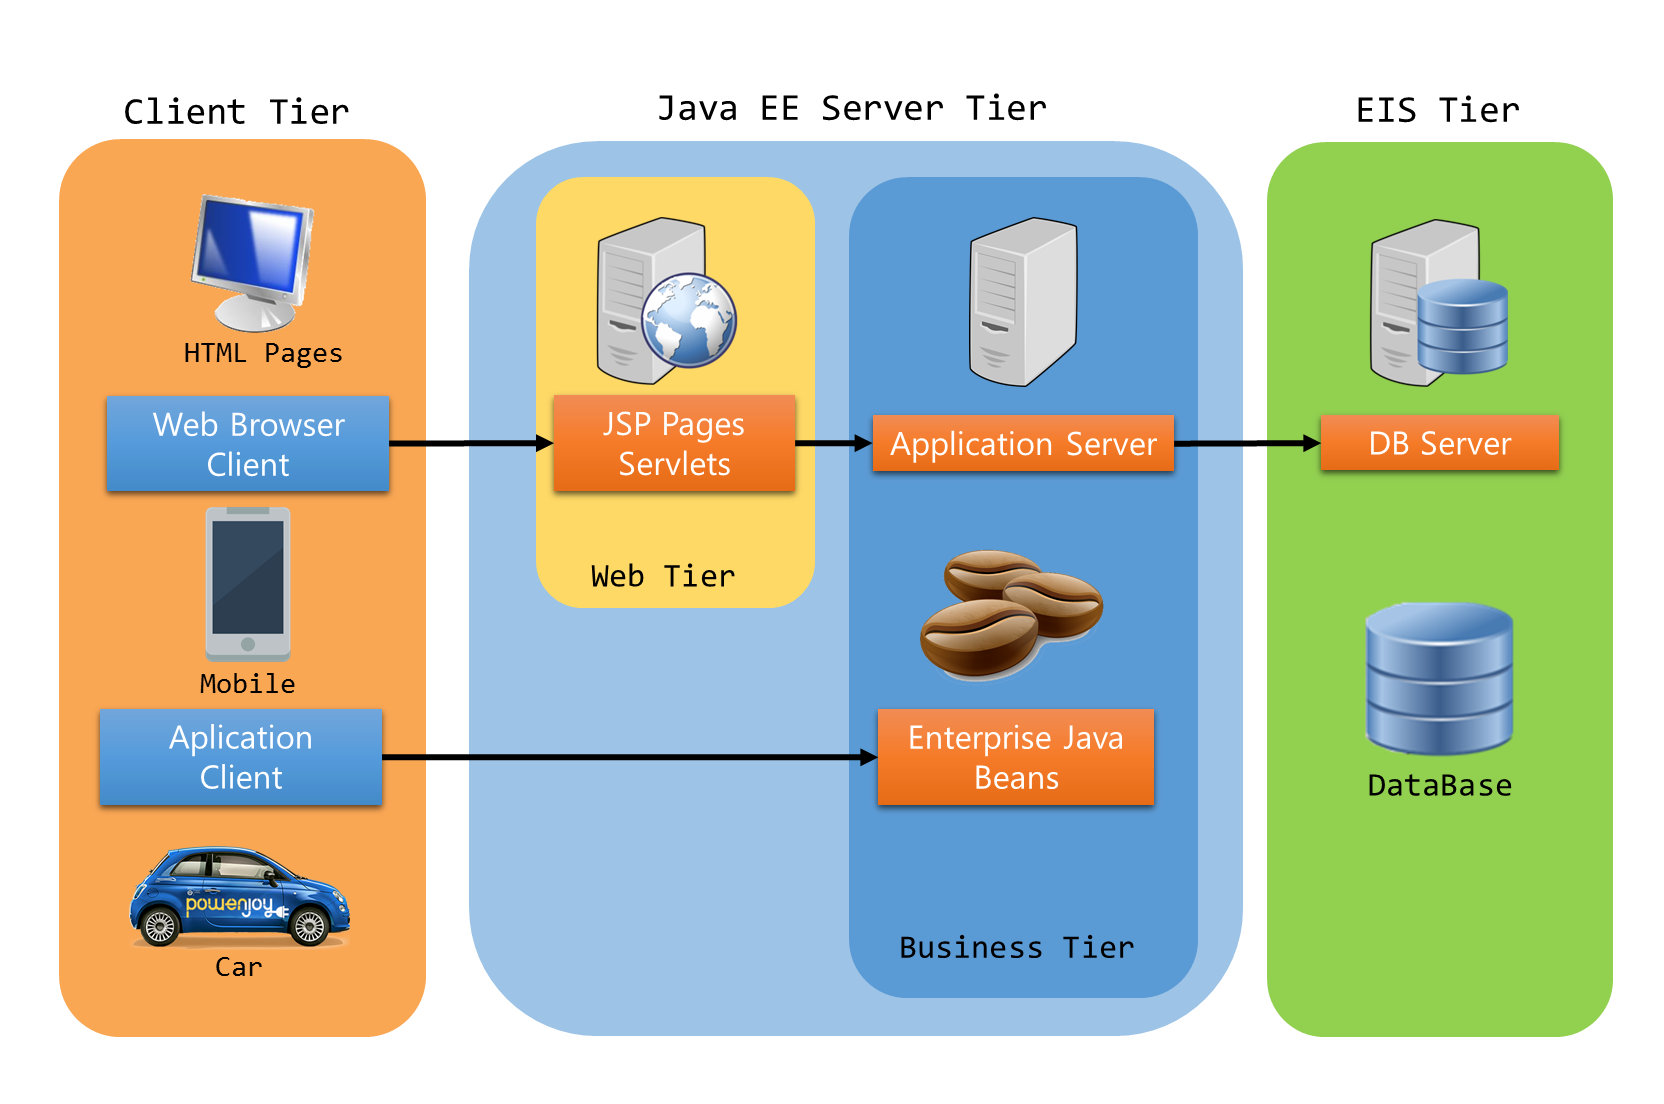
\includegraphics[width=1.35\textwidth]{ProposedSystem.png}}%
\caption {Proposed System Architecture}
\vspace*{0.5cm}
\end{figure}
\newpage

\section{Actors}
\subsection{User}
Is the Main Actor of our service. Any person that once Registered can take advantage of the features of the PowerEnJoy service.
\subsection {CRM}
Customer Relationship Manager, will interface with the User in case of any problem that may arise and can intervene in the System to fix any issues. His permissions in the System include but are not limited to check on every Car of the service, perform or cancel any Reservation, modify the fee of an User's ride in case of a confirmed major cause, change the Status of a Car and execute a Transaction to a User post-ride.

\section{Requirements}
\subsection{Functional Requirements}
\subsubsection{\textbf{User Requirements:}}
\begin{description}
\item [G.1)]First-Time Users must be able to register to the System creating an Account. 
\begin{itemize}
	\item[-]The System must allow an user that has not created an Account to register by providing valid credentials, an e-mail and payment information.
	\item[-]The System must sent a password to the Registered User Email that can be used to Log into the Account.
\end{itemize}
\item [G.2)]Registered Users must be able to login to their Account at any time they want.
\begin{itemize}
	\item[-]The System must allow Registered Users to log into their Account only if they provide their correct e-mail and password.
\end{itemize}
\item [G.3)]Users can save his/hers credentials in the System.
\begin{itemize}
	\item[-]The System must be able save Users credentials upon theis request.
	\item[-]When the user choose to save his/her credential they don't need to inform it in every time they open the System.
\end{itemize}
\item [G.4)]A Registered User will be able to make a Reservation of any available Car near his/her current location or from an address that she/he can specify.
\begin{itemize}
	\item[-]The System must be able to locate the User via GPS.
	\item[-]The System must allow the Users to enter a determined address, in case they don't want to use their current location to locate the cars in the area.
	\item[-]The System must be able to locate all available Cars via GPS.
	\item[-]The System must show the User all the available Cars near the user given location.
	\item[-]The System must allow the Users to select one of the Cars showed to them to create a Reservation, the selected Car will be marked as reserved.
\end{itemize}
\item [G.5)]Users that have made a Reservation must be able to notify the System when they are nearby the Reserved Car so the System can unlock it.
\begin{itemize}
	\item[-]While a Reservation is active, the System must allow the User to notify that they are nearby their Reserved Car.
	\item[-]The System must confirm the notification by checking that the User current location and the Car location coincide.
	\item[-]The System must unlock the Reserved Car and set it to Ready to Use.
\end{itemize}
\item [G.6)]A User that has made a Reservation must be able to cancel it before 1 hour starting from the time when the Reservation was made.
\begin{itemize}
	\item[-]The System must check how long has passed from the reservation time, if it less then one hour the user will be able to open the reservation and cancel it without being charged for it.
	\item[-]The System must confirm the user request and set the car as available again.
\end{itemize}
\item [G.7)]In case an User hasn't started using the Reserved Car at 45 minutes after the Reservation was made, he/she will be notified that either if the Reservation is not canceled or the Car is not used in 15 minutes, the Reservation will be automatically canceled and a 1 Euro fee will be charged to her/his Account.
\begin{itemize}
	\item[-]After 45 minutes from the reservation time has passed, the System must send a notification to the user's registered smartphone warning that he/she has 15 minutes left to pick up the car or to cancel the reservation.
	\item[-]After the full hour has passed and the reservation is still active, the System must cancel the reservation, block this user account for the next hour and charge the fee of 1 Euro for not picking up the car.
\end{itemize}
\item [G.8)]When Users start using their Reserved Car, they must be able to see their current expenses on the service through a System screen inside the Car.
\begin{itemize}
	\item[-]The car System must keep track of the gross fee to be paid by the user.
	\item[-]As soon as the car ignites, the car System must start showing the fee on the computer monitor and keep it this way until the user is finished using the car.
\end{itemize}
\item [G.9)]The User must be able to know where the safe parking areas are nearby his/her current location or any address that she/he can specify.
\begin{itemize}
	\item[-]The System must be able to show, when requested, a map with the safe parking zones and points with eletricity plugs .
\end{itemize}
\item [G.10)]Users must be able to finish their use of the Car when leaving it in a Safe Parking Area and exiting the car. The User will then be charged for the use of the service. The used Car will be locked and freed for Users to be reserved.
\begin{itemize}
	\item[-]The System must verify if the car is parked in a Safe Parking Area. If the car isn't located in one, the System must notify the user on the screen of the car that it's not possible to finish the ride.
	\item[-]The System must show a message on the car's screen asking if the user want to finish the ride or if want to continuing the use of the car.
	\item[-]The user must answer to the request. If the user want to keep using it, the System will set the car as reserved for one hour. Nevertheless in terms of payment the System will charge the same amount of money in the final Transaction as if the car has been in a ride. If the user does not want to use the car the System will finish ride.
	\item[-]Upon the user leaving of the car the System must lock the car and consider the user's answer to whether set the car as available or reserved.
\end{itemize}
\item [G.11)]The User will always be notified when any Transaction is made on his Account.
\begin{itemize}
	\item[-]The System must notify the user of every Transaction made on his Account by email. Further information related to the ride as the total time, the driven route and the charged Fees must compose the email.
\end{itemize}
\item [G.12)]Notify the Users that are currently using a Car of any available discounts on their ride if they abide by the 'Virtuous Behaviour Rules' and of the extra fee in case of not respecting the facilitation of the re-charging of the Car on site. These extra discounts/charges will be applied on the Total fee at the end of the ride.
\begin{itemize}
	\item[-]The System must notify the user on the Car's screen of the any information related with a discount or extra fee.
  	\item[-]The System must calculate at the end of the ride if any discount or extra fee is applicable. These fees are:
	\item [G.12.1)]Apply a 10\% discount if the User takes at least 2 other passenger into the car.
	\begin{itemize}
	\item[-]The System must read from the status of the Car the number of passengers and if it's 2 or more, apply the 10\% discount to the ride fee.
	\end{itemize}
	\item [G.12.2)]Apply a 20\% discount if the User leaves the Car with the battery at least half-full.
	\item [G.12.5)]Apply a 30\% extra fee if the User leaves the Car with the battery less than 20\% full.
	\begin{itemize}
	\item[-]The System must read from the status of the Car the amount of battery left and if it's 50\% or more calculate the 20\% discount else if it's less than 20\% calculate the 30\% extra fee.
	\end{itemize}
	\item [G.12.3)]Apply a 30\% discount if the User leaves and plugs the Car in a Re-Charging Station.
	\begin{itemize}
	\item[-]The System must detect from the status of the Car if it's plugged in to a Re-Charging Station and if it is, calculate the 30\% discount.
	\end{itemize}
	\item [G.12.4)]Apply a 30\% extra fee if the User leaves the Car at more than 3KM from the nearest Re-Charging Station.
	\begin{itemize}
	\item[-]The System must read from the status of the Car its current location and the distance to the nearest Re-Charging Station, if it is more than 3KM then calculate the 30\% extra fee.
	\end{itemize}
	\item[-]The System must apply these discounts or extra fees at the end of the ride over the total fee.
\end{itemize}

\item [G.13)]Users can activate the `Money Saving'a option on their Account to be notified of any nearby Re-Charging station on their arrival destination. Leaving the car at the end of the ride at this station and plugging it will register as a 'Virtuous Behavior' and will apply and extra discount when charging the User.
\begin{itemize}
	\item[-]Users must be allowed to enable the 'Money Saving' option on their accounts at any time they choose.
	\item[-]The System must allow the user to input his/her destination at any time of the ride whether on the app or on the car's screen.
	\item[-]Upon the final destination of the user the System must direct the end of the ride considering a uniform distribution of parked cars of the System, the nearest charging station in relation with the address informed and  the availability of these charging stations.
\end{itemize}
\item [G.14)]Users must have the option to contact a CRM at any moment, the System must provide a Customer Service area that offers a Chat feature within the App or a phone number.
\begin{itemize}
	\item[-]The System must show a Customer Service number in its Customer Service Area.
	\item[-]The System must have a Chat feature that will allow the User contact directly a CRM.
\end{itemize}
\end{description}

\subsubsection{\textbf{CRM Requirements:}}
\begin{description}
\item [G.15)]CRM must be able to log in into the System and see a list of all the Cars available, reserved, in use or unavailable.
\begin{itemize}
	\item[-]The System must allow log in to CRM if they have provided valid username and password.
	\item[-]The System must show to CRM a list of all the Cars that can be sorted by Status.
\end{itemize}
\item [G.16)]CRM has to be able to receive User Reports via chat or outside the app via phone call and be able to register it to the System.
\begin{itemize}
	\item[-]When a User uses the Chat feature to contact a CRM the System will redirect the chat to the first available CRM and notify him/her that a User is contacting her/him.
	\item[-]The System must allow the CRM to create a User Report that will link a User with a Car and if necessary allow the option to add a Transaction.
\end{itemize}
\item [G.17)]CRM upon request form an User or any major cause can Reserve or cancel any active Reservation.
\begin{itemize}
	\item[-]The System must allow from the list of all Cars showed to the CRM, the option to Reserve any available Car for a User or cancel a Reservation of a Reserved Car. This action does not include a User Report.
\end{itemize}
\item [G.18)]CRM must be able to change the Status of a Car given a User Report and tag it, in case it's unavailable, if it's due to Re-Charge, Fix, or Removal.
\begin{itemize}
	\item[-]The System must allow from the list of all Cars showed to the CRM, the option to Reserve any available Car for a User or cancel a Reservation of a Reserved Car. This action does not include a User Report.
\end{itemize}
\item [G.19)]Upon the completion of an User Report CRM must be able to apply extra fees or refund the payment to any User in case the situation demands it.
\begin{itemize}
	\item[-]The System at the end of an User Report must ask for confirmation of the CRM in case the Report includes a Transaction. This can be an extra fee that the User must pay or a refund the service owns the User.
\end{itemize}
\end {description}

\subsection{Non Functional Requirements}
\subsubsection{User Interface}
For our User Interface (UI) we'll offer a mobile App for Users and a desktop web App for Users and CRM. They will offer:
\begin {itemize}
\item \textbf{LogIn Page:} First screen of the app with the LogIn and SignIn options.
\begin{figure}[h]
\centering
\vspace*{\fill}
\noindent\makebox[\textwidth]{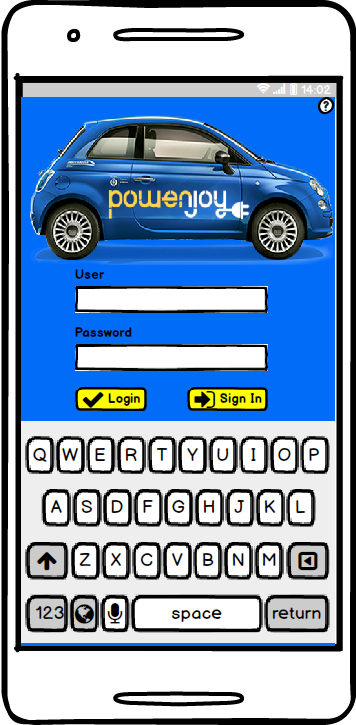
\includegraphics[width=0.28\textwidth]{1.png}}%
\caption {UI LogIn Page}
\vspace*{0.2cm}
\end{figure}
\pagebreak
\item \textbf{Main Page:} Main page of the app where the user sees the map his location and selects the available cars. In Case of CRM, it can see all Cars.
\begin{figure}[h]
\centering
\vspace*{\fill}
\noindent\makebox[\textwidth]{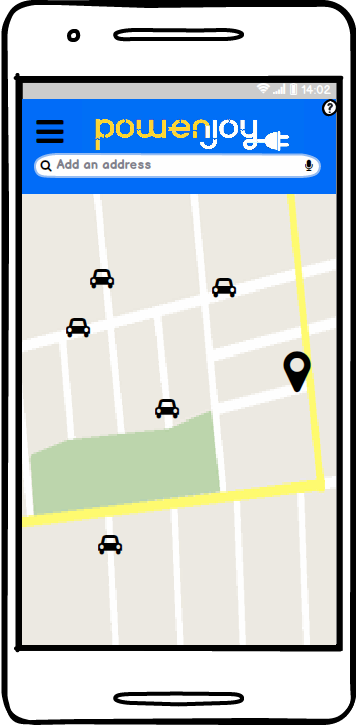
\includegraphics[width=0.28\textwidth]{2.png}}%
\caption {UI Main Page}
\vspace*{0.2cm}
\end{figure}
\item \textbf{Car Details Page:} Once a Car is selected this page allows to reserve a car and contais informations for the decision.
\begin{figure}[h!]
\centering
\vspace*{\fill}
\noindent\makebox[\textwidth]{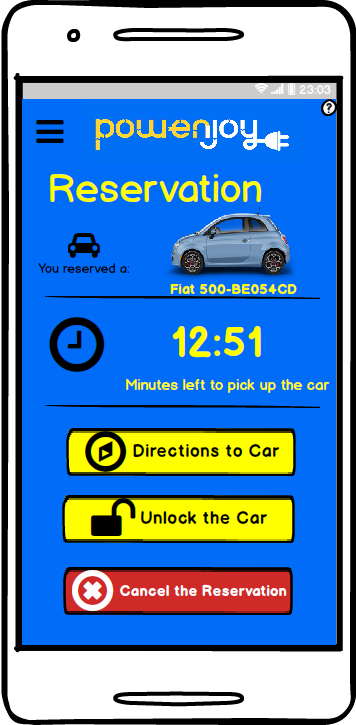
\includegraphics[width=0.28\textwidth]{4.png}}%
\caption {UI Car Details Page}
\vspace*{0.2cm}
\end{figure}
\pagebreak
\item \textbf{Reservation Page:} Once the Reservation is made, the User can see the details of her/his Reservation and have the option to cancel it.
\begin{figure}[h!]
\centering
\vspace*{\fill}
\noindent\makebox[\textwidth]{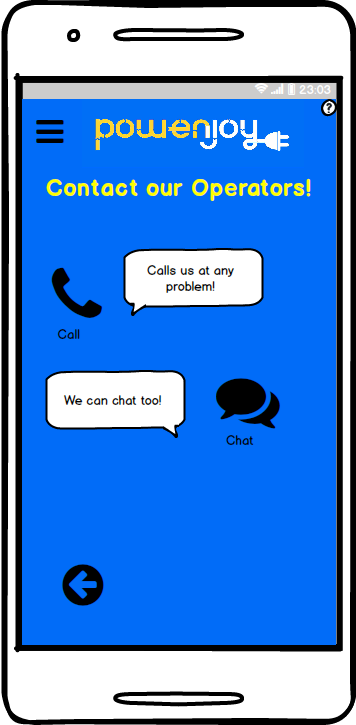
\includegraphics[width=0.28\textwidth]{5.png}}%
\caption {UI Reservation Page}
\vspace*{0.2cm}
\end{figure}
\item \textbf{Ride Page:} Once a Ride started this page shows the details of the current ride, it's present also in the Car screen App.
\begin{figure}[h!]
\centering
\vspace*{\fill}
\noindent\makebox[\textwidth]{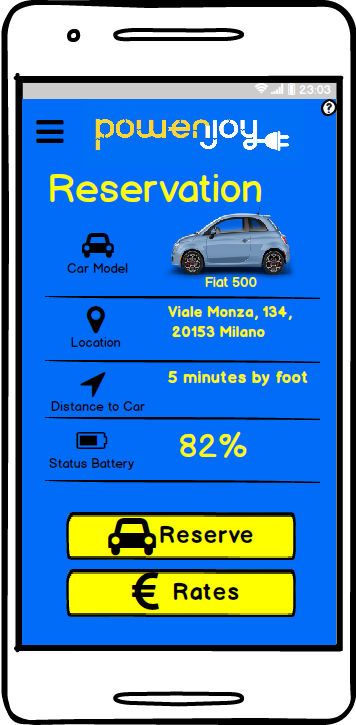
\includegraphics[width=0.36\textwidth]{3.png}}%
\caption {UI Mobile Ride Page}
\vspace*{0.2cm}
\end{figure}
\pagebreak
\begin{figure}[h!]
\centering
\vspace*{\fill}
\noindent\makebox[\textwidth]{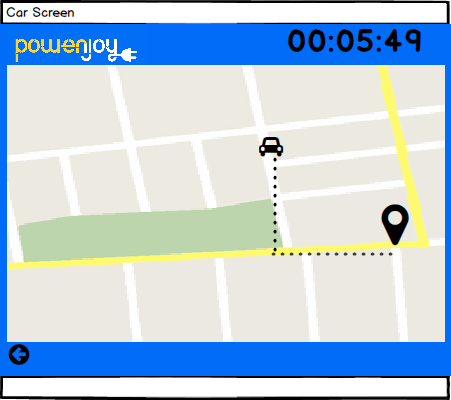
\includegraphics[width=0.7\textwidth]{CarScreen.png}}%
\caption {UI Car Ride Page.}
\vspace*{0.2cm}
\end{figure}
\item \textbf{Email Page:} While not part of the App UI, the System should respond with an email to the User at the end of the Ride showing the final details for it.
\begin{figure}[h!]
\centering
\vspace*{\fill}
\noindent\makebox[\textwidth]{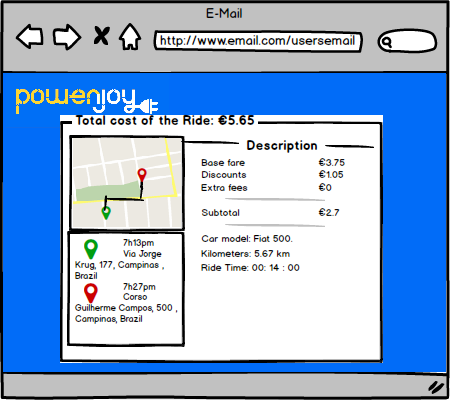
\includegraphics[width=0.7\textwidth]{EmailUser.png}}%
\caption {UI Email Page}
\vspace*{0.2cm}
\end{figure}
\pagebreak
\item \textbf{Contact Page:} Page where the User can contact the CRM operator.
\begin{figure}[h!]
\centering
\vspace*{\fill}
\noindent\makebox[\textwidth]{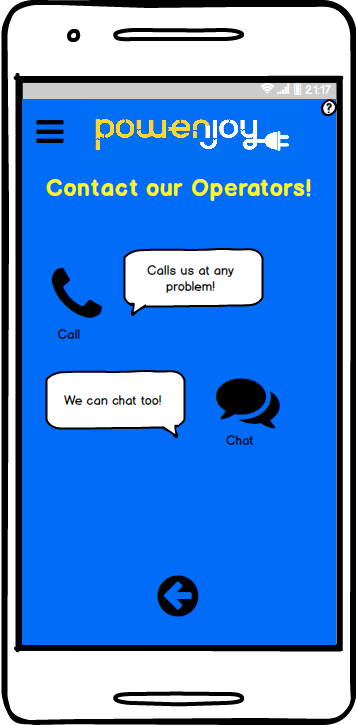
\includegraphics[width=0.28\textwidth]{6.png}}%
\caption {UI Contact Page}
\vspace*{0.2cm}
\end{figure}

\end{itemize}
\subsubsection{Documentation}
To organize this project workflow and development the following Documents will be drafted:
\begin {itemize}
\item Requirements And Specifications Document (RASD): Describes the Goals of the project and how to achieve them by specifying the Requirements.
\item Design Document (DD): Defines the real structure of the System. Architecture, Components and design decisions will be explained here.
\item Project Testing Document: Will detail the Test process for the system before deployment. Test case specifications, procedues, incident, reports will be considered Documentation Testing.
\item Project Management Documentation: Specific assignment of tasks, stimations and goals for each of the development phases.
\end{itemize}

\newpage
\subsubsection{System Architecture}
Project will be developed using a JEE Platform based in a 3-Tier Client/Server Architecture. First idea consists in a Distributed Logic structured layers where the Client Apps will interface with the Server that will store the logic and will connect with the Data Layer of the System. The architecture as explained briefly in the \textbf{\hyperref[sec:propSystem]{Proposed System}} section will consist of:
\begin {itemize}
\item Client Tier: 
\begin {itemize}
\item [-]Web Client on a browser with abilitated JavaScript for the Web App use. 
\item [-]Application Client for the Mobile App (Android and iOS), with GPS functionalities. We will consider the screen present in the Car as a Client App of the System that'll implement some logic to interface to the Car Software to Lock, Unlock, read the Battery level and other functions.
\end{itemize}

\item Server Tier:
\begin {itemize}
\item [-]Web Server that'll answer connections for Web Clients. It will interface with the Application Server.
\item [-]JavaEE Application Server, that'll implement the logic of the System. Application Clients (Users and Cars) will connect directly to it. Will implement JavaBeans to handle request from multiple Clients at a time.
\end{itemize}

\item Enterprise Information System (EIS) Tier:
\begin{itemize}
\item [-]DataBase Server, accessed by the Application Server to store all the data refering to the System.
\end{itemize}

\end{itemize}

\subsubsection{Hardware Consideration}
As stated in the Architecture Considerations we'll need a server able to store our Application and DataBase and be accessible by multiple Clients at a time. We'll consider the Server to be always accesible through an stable connection to Internet. 
As an extension of the System we have the Clients running in the Cars, they'll need to be accessible via 3G and have GPS feature for localization.

\subsubsection{Incident Handling}
We'll consider our data to be persistent. If by any case any data is lost or corrupted we expect not to create big losses to the System, all transactions of data will be considered atomic we expect no loss during any kind of transaction. 

\subsubsection{Security}
Data Backups will be considered daily for data security. Accounts will be protected by hashed passwords. As one of the requirements of the project asked to send Users a password via mail we assume that it'll be handled by secure servers (IMAPS) so we're assured just the User can see it. Firewalls will be considered for our Servers connections. In case of breach, User Accounts can be blocked by CRMs. CRM Accounts are introduced directly into the DataBase by a separate system that register the Company employees, we assume it safely as well.

\section{Scenario Identifying}

\begin{tabular}{ |  l  |   l |  l  |  }
\hline
	\textbf { \textbf{Scenario}} & Carol is a First-Time User\\ \hline
	 \textbf{Actor}& User\\ \hline
	\textbf{Background conditions}&\parbox[t]{8cm}{Carol do not have an Account but she wants to create one. } \\ \hline
	\textbf{Flux of events} & \parbox[t]{8cm}{\textbullet  Carol selects the sign-up option on the App;\\\textbullet The System shows a form where Carol can insert her data;\\\textbullet Carol inserts her credentials, email and the payment information and finishes the process;\\\textbullet  The System checks the consistence of the data;\\\textbullet  The System informs Carol of the success of the registration;}\\ \hline
	\textbf{Exit conditions} &\parbox[t]{8cm}{ System confirms the creation of a new user and send an email to the user's email address informing the password and confirming the registration.}\\ \hline
	\textbf{Exception} & \parbox[t]{8cm}{Carol inserts data that the System can't validate. System can not finish operation until Carol inserts the correct data.   }\\ \hline
\end{tabular}
\newline

\begin{tabular}{ |  l  |   l |  l  |  }
\hline
	\textbf { \textbf{Scenario}} & Alex wants to reserve the nearest car\\ \hline
	 \textbf{Actor}& User\\ \hline
	\textbf{Background conditions}&\parbox[t]{8cm}{Alex is Registered User. He is a heavy user of the service, and to save time he had saved his credentials in the app to open it without the need of a login. } \\ \hline
	\textbf{Flux of events} & \parbox[t]{8cm}{\textbullet  Alex open the App;\\\textbullet  The System redirects to the Main Page;\\\textbullet By experience Alex manually search in the map for the nearest car;\\\textbullet Alex find one car select and reserves it;\\\textbullet 	The System reserve the car;\\\textbullet  Alex walks in the direction of the location of the reserved car; }
  \\ \hline
	\textbf{Exit conditions} &\parbox[t]{8cm}{ The System confirms the reservation of the car that Alex had selected.}\\ \hline
	\textbf{Exception} & \parbox[t]{8cm}{The saved credentials are not valid and the login fail.\\
The car that Alex selects is already reserved and the System can not effectuate the reservation.
}\\ \hline

\end{tabular}
\newline
\begin{tabular}{ |  l  |   l |  l  |  }
\hline
	\textbf { \textbf{Scenario}} & \parbox[t]{8cm}{Francesco wants to login to see available cars without doing a reservation}\\ \hline
	 \textbf{Actor}& User\\ \hline
	\textbf{Background conditions}&\parbox[t]{8cm}{Francesco is a Registered user.\\He is a new user and want to explore the functions of the System. } \\ \hline
	\textbf{Flux of events} & \parbox[t]{8cm}{\textbullet  Francesco open the app and login;\\\textbullet Francesco try to find a car manually searching in the map, but he does not like of searching by himself;\\\textbullet Francesco open the side menu and find the option 'Search for a car', he selects it;\\\textbullet The System automatically search for the nearest car based on Francesco's location;\\\textbullet 	The System find the finds a car and trace the route in the map of the App's map;\\\textbullet  Francesco satisfied to know this functionality of the app and closes it without reserving a car; }
  \\ \hline
	\textbf{Exit conditions} &\parbox[t]{8cm}{ The System allows the user to search for the available cars without the need of a reservation.}\\ \hline
	\textbf{Exception} & \parbox[t]{8cm}{The login fail.\\The System does not find available cars and can't return results for the search.

}\\ \hline
\end{tabular}
\newline
\begin{tabular}{ |  l  |   l |  l  |  }
\hline
	\textbf { \textbf{Scenario}} & \parbox[t]{8cm}{Mario is doing overtime. He knows that the metro stops at 0h so he wants to reserve a car near the metro station. He'll exit at 0h20.}\\ \hline
	 \textbf{Actor}& User\\ \hline
	\textbf{Background conditions}&\parbox[t]{8cm}{Mario is a Registered user.\\He uses the System occasionally.} \\ \hline
	\textbf{Flux of events} & \parbox[t]{8cm}{\textbullet  It's 23h50. Mario open the App and login;\\\textbullet The System redirects to the Main Page where there is an option to inform an address to find a car;\\\textbullet Mario inform the address of the metro;\\\textbullet The System return the metro station location;\\\textbullet  Mario see the available cars selects one and reserve it;} \\ \hline
	\textbf{Exit conditions} &\parbox[t]{8cm}{ The System reserves the car selected by the user and assure reservation for a period of one hour.}\\ \hline
	\textbf{Exception} & \parbox[t]{8cm}{The login fail.\\There is no available car in the address that Mario and he does not reserve a car.}\\ \hline
\end{tabular}
\newline
\begin{tabular}{ |  l  |   l |  l  |  }
\hline
	\textbf { \textbf{Scenario}} & \parbox[t]{8cm}{Angela is walking back home when she sees a car parked by her side. She wants to unlock it to drive back home.}\\ \hline
	 \textbf{Actor}& User\\ \hline
	\textbf{Background conditions}&\parbox[t]{8cm}{Angela is a Registered user.\\She did not make a reservation of the car that she wants to drive. } \\ \hline
	\textbf{Flux of events} & \parbox[t]{8cm}{\textbullet  Angela open the App and do the login;\\\textbullet The System redirects to the Main Page;\\\textbullet Angela immediately finds the car, that is beside her location;\\\textbullet She selects the car and request a reservation;\\\textbullet The System reserves the car;\\\textbullet Angela proceeds to unlock the car in the App; \\\textbullet The System checks the reserve and the current position of the User and the Car;\\\textbullet The System unlocks the car and set it for Ready to Use mode;\\\textbullet Angela get in the car and drives home;} \\ \hline
	\textbf{Exit conditions} &\parbox[t]{8cm}{ System reserves the car and unlock it upon User location.}\\ \hline
	\textbf{Exception} & \parbox[t]{8cm}{The login fail.\\The car that is besides Angela is already reserved so she can't reserve the car for her use in the moment.
}\\ \hline
\end{tabular}
\newline
\begin{tabular}{ |  l  |   l |  l  |  }
\hline
	\textbf { \textbf{Scenario}} & \parbox[t]{8cm}{Sarah wants to cancel a reservation}\\ \hline
	 \textbf{Actor}& User\\ \hline
	\textbf{Background conditions}&\parbox[t]{8cm}{Sarah is a Registered User.\\She does not need to get the car anymore so she wants to cancel the reservation that she made 30 minutes ago. } \\ \hline
	\textbf{Flux of events} & \parbox[t]{8cm}{\textbullet  Sarah open the App and do the login;\\\textbullet Sarah selects in the menu of the App the option 'My reservation';\\\textbullet The System shows Sarah's reservation;\\\textbullet Sarah see the status of the reservation;\\\textbullet Sarah selects the option of canceling the reservation;\\\textbullet The System checks the time that Sarah did the reservation, verifies that is possible to cancel the ride and proceeds to do this operation;} \\ \hline
	\textbf{Exit conditions} &\parbox[t]{8cm}{ The System verifies if the reservation's time is under 1 hour if so the user can cancel the reservation.}\\ \hline
	\textbf{Exception} & \parbox[t]{8cm}{The login fails.\\
Sarah tries to cancel the reservation after one hour period  of reservation and System does not allow Sarah cancel the reserve.
}\\ \hline
\end{tabular}
\newline
\begin{tabular}{ |  l  |   l |  l  |  }
\hline
	\textbf { \textbf{Scenario}} & \parbox[t]{8cm}{Paulo is late to pick up the reserved car.}\\ \hline
	 \textbf{Actor}& User\\ \hline
	\textbf{Background conditions}&\parbox[t]{8cm}{Paulo is a Registered User.\\He had reserved a car. It has passed 45 minutes.} \\ \hline
	\textbf{Flux of events} & \parbox[t]{8cm}{\textbullet  Paulo have 15 minutes left to pick the reserved car; \\\textbullet The System emits an alert in the App informing that Paulo is running out of time;\\\textbullet  Paulo sees the alert and rushes into the location where the car is parked;} \\ \hline
	\textbf{Exit conditions} &\parbox[t]{8cm}{ The System emits an alert when the period of the car's reserve is ending.}\\ \hline
	\textbf{Exception} & \parbox[t]{8cm}{The alert fails.\\ Paulo don't see the alert.\\
Paulo couldn't make to the car in 15 minutes and the System automatically cancel the reservation, charges 1 euro of Paulo's account and will not allow Paulo to reserve a car for 1 hour.
}\\ \hline
\end{tabular}
\newline
\begin{tabular}{ |  l  |   l |  l  |  }
\hline
	\textbf { \textbf{Scenario}} & \parbox[t]{8cm}{Hugo is about to finish a ride.}\\ \hline
	 \textbf{Actor}& User\\ \hline
	\textbf{Background conditions}&\parbox[t]{8cm}{Hugo is a Registered User.\\He was driving into a unknow direction.} \\ \hline
	\textbf{Flux of events} & \parbox[t]{8cm}{\textbullet  At some point Hugo decides to stop the car;\\\textbullet He finds parking spot and proceeds to park the car;\\\textbullet Hugo finishes the maneuver and turn off the car; \\\textbullet The System verifies if the parking spot is in some Safe Park Area and proceeds to finish the ride;\\\textbullet The System shows an interface on the car's screen asking if Hugo will finish the ride; \\\textbullet Hugo selects that he will finish the ride; \\\textbullet Hugo left the car;\\\textbullet The System finish the ride and lock the car;} \\ \hline
	\textbf{Exit conditions} &\parbox[t]{8cm}{ The System verifies the Status of the car and   proceeds to finish Hugo's ride sending to his email the information of the ride as the route and the transaction.}\\ \hline
	\textbf{Exception} & \parbox[t]{8cm}{Hugo park the car in a no Safe Park Area, and the System can not finish the ride.}\\ \hline
\end{tabular}
\newline
\begin{tabular}{ |  l  |   l |  l  |  }
\hline
	\textbf { \textbf{Scenario}} & \parbox[t]{8cm}{Marina wants to use the System in the most economical way.}\\ \hline
	 \textbf{Actor}& User\\ \hline
	\textbf{Background conditions}&\parbox[t]{8cm}{Marina is Registered User and she had saved her credentials on the app.\\She had just unlocked the car and is about to begin the ride.} \\ \hline
	\textbf{Flux of events} & \parbox[t]{8cm}{\textbullet  Marina has a previous knowledge of the 'Money Saving' option so when she got in the car she informs in car's screen map her destination;\\\textbullet The System calculates the optimal destination considering the distribution of the cars in the city, the available plugs and the destination address;\\\textbullet The System return options of parking spots to Marina; \\\textbullet She considers these options and selects one. She starts the ride following the GPS route of the car's screen;\\\textbullet Mariana drives to the destination;\\\textbullet Marina turn of the car;\\\textbullet The System show a question on the car's screen asking if Marina will finish the ride;\\\textbullet Marina selects that she will finish the ride; \\\textbullet  The System show a message on the saying that Marina is besides the plug and advice to connect the car to the plug;\\\textbullet Marina left the car and proceeds to connect the plug into the car; \\\textbullet The System finish the ride and lock the car; } \\ \hline
	\textbf{Exit conditions} &\parbox[t]{8cm}{ The System verifies the Status of the car and proceeds to finish Marina's ride sending to his email the information of the ride as the route and the transaction.}\\ \hline
	\textbf{Exception} & \parbox[t]{8cm}{The System can not return a destination due the lack of the available Re-Charging Stations in relation with the distribution of the cars.  }\\ \hline
\end{tabular}
\newline
\newline
\begin{tabular}{ |  l  |   l |  l  |  }
\hline
	\textbf { \textbf{Scenario}} & \parbox[t]{8cm}{The Car that Julia was driving had mechanical problems during the Ride.}\\ \hline
	 \textbf{Actor}& User, CRM operator\\ \hline
	\textbf{Background conditions}&\parbox[t]{8cm}{Julia is Registered User and she had saved her credentials on the app. She was driving a Car when it suddenly stops.} \\ \hline
	\textbf{Flux of events} & \parbox[t]{8cm}{\textbullet  Julia open the App;\\\textbullet She selects the option 'Problems with the Car';\\\textbullet The System immediately provides an option whether to chat or call to an CRM operator; \\\textbullet Julia chooses to call and the System redirects to the dialing process;\\\textbullet The calling established a connection of Julia and the CRM operator;\\\textbullet Julia describe the situation to the CRM operator;\\\textbullet The CRM operator finishes the Julia's ride, check if there is any extra charging in the Transaction of the riding and set the car as unavailable;\\\textbullet Julia finishes the call and left the car;} \\ \hline
	\textbf{Exit conditions} &\parbox[t]{8cm}{ The CRM operator directs the relation when between the User and the System in such events and is enable to finish the ride and to set the car as unavailable.}\\ \hline
	\textbf{Exception} & \parbox[t]{8cm}{The saved credentials are not valid and the login fail.\\
The connection between the CRM operator and the User fails.\\
There is no CRM operator available;\\
The CRM operator could not identity the problem with the Car. 
}\\ \hline
\end{tabular}

\begin{tabular}{ |  l  |   l |  l  |  }
\hline
	\textbf { \textbf{Scenario}} & \parbox[t]{8cm}{Frederico had a medical condition and could not pick up the reserved car}\\ \hline
	 \textbf{Actor}& User, CRM operator\\ \hline
	\textbf{Background conditions}&\parbox[t]{8cm}{Frederico is a Registered user and had made and missed a reservation.He had an accident and was unable to get the car.} \\ \hline
	\textbf{Flux of events} & \parbox[t]{8cm}{\textbullet  Frederico open the app and do the login;\\\textbullet He chooses the option 'Talk with us' and call for the CRM operator\\\textbullet The calling established a connection of Frederico and the CRM operator;\\\textbullet Frederico explains the case to the CRM operator;\\\textbullet The CRM operator analyses the case and apply some alterations on the system such as canceling the charged fee in one Transaction of Francesco's Account;\\\textbullet Frederico finishes the call;} \\ \hline
	\textbf{Exit conditions} &\parbox[t]{8cm}{ CRM operator analyses Frederico's request and apply or not changes is the system following these requests}\\ \hline
	\textbf{Exception} & \parbox[t]{8cm}{The login fail.\\
	The connection between the CRM operator and the User fails.\\
There is no CRM operator available;\\
The CRM operator could not apply the changes upon the user's request.
}\\ \hline
\end{tabular}

\newpage

\section{UML Modeling}
\subsection{Use Case Diagram}
Use case Diagram represents all the situations available to Users explained in the Scenarios.
\begin{figure}[h]
\centering
\vspace*{\fill}
\noindent\makebox[\textwidth]{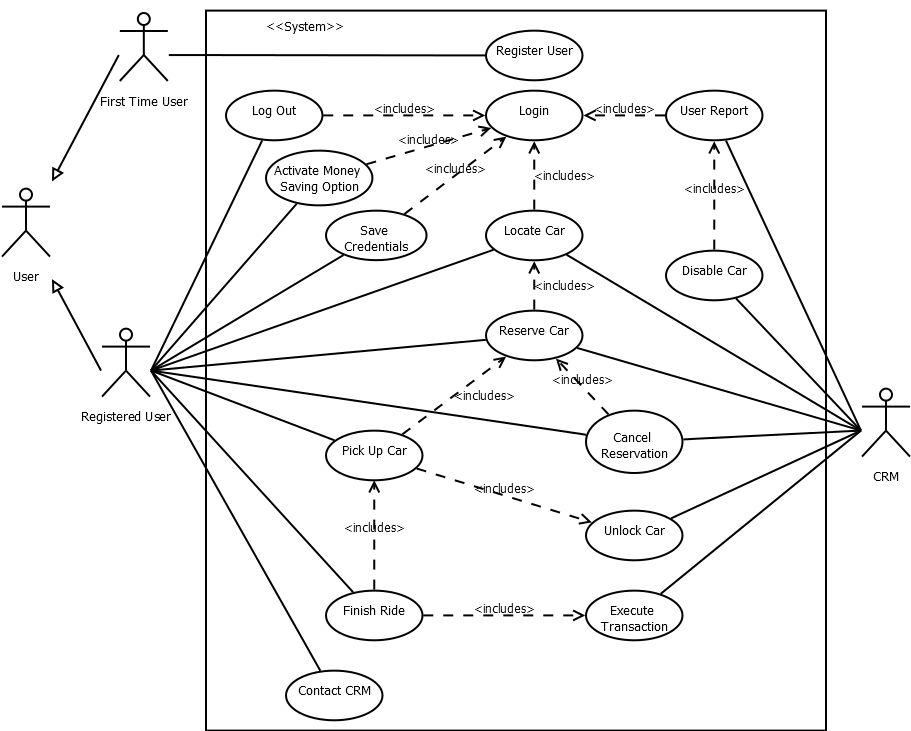
\includegraphics[width=1.35\textwidth]{UseCaseCRM.png}}%
\caption {Use Case Diagram}
\vspace*{2cm}
\end{figure}
\newpage

\subsubsection{Use Cases Description}
Use Cases derived from the Scenarios previously detailed and based on the Use Case Diagram.
\begin{center}
\rule{8cm}{0.4pt}
\end{center}
\textbf{Use Case:} First Time User Registers.
\newline
\textbf{Actors:} User
\newline
\textbf{Flow of Events:}
\begin{itemize}
\item User selects the Sign-Up option on the App.
\item A form is presented to the User where he/she can fill her/his information.
\item The User inserts all credentials and valid payment options and proceeds with the operation.
\item The System informs the User the success of the Registration.
\end{itemize}
\textbf{Exit Conditions:} The System confirms the creation of the new User and adds its Account to the Database. An email with the User's Password is sent for her/him to Log in.
\newline
\textbf{Exceptions:} The User inserts invalid data so the System can't confirm the Registration.
\newline

\begin{center}
\rule{8cm}{0.4pt}
\end{center}
\textbf{Use Case:} User Reserves and Rides a Car.
\newline
\textbf{Actors:} User
\newline
\textbf{Flow of Events:}
\begin{itemize}
\item User Logs In to the App in a mobile device.
\item User sees in the Main Page the map with the available Cars near the User current Location.
\item User selects a Car and reserves it.
\item The System creates a Reservation with the User and the Car, maked now as reserved.
\item User moves toward the Location of the Reserved Car and ask the System to unlock it.
\item The System confirms that the User and the Car location are the same and unlocks the Car.
\item As soon as the User ignites the Car the System starts the registration of the Ride.
\item The User arrives to the desired destination and parks the Car in a Safe Parking Area.
\item The System asks the User if he/she desires to finish the Ride.
\item When the User confirms, the System ends the Ride and charges its fee to the User Account. 
\end{itemize}
\textbf{Exit Conditions:} The System verifies the Status of the Car and sends an email to the User with the information of the ride as the route and the Transaction.
\newline 
\textbf{Exceptions:} The User cannot find an available Car, the User cancels the Reservation or the User does not park in a Safe Parking Area, thus the System cannot end the Ride.
\newline

\begin{center}
\rule{8cm}{0.4pt}
\end{center}
\textbf{Use Case:} User asks to cancel a Reservation.
\newline
\textbf{Actors:} User, CRM
\newline
\textbf{Flow of Events:}
\begin{itemize}
\item User makes a Reservation for a Car.
\item After some time before the one hour limit has passed the User decides to cancel the Reservation
\item Instead of canceling the Reservation with the App the User decides to call the Customer Service Number.
\item A CRM answers the User an after confirming his/her information is correct, looks for the Reservation in the System.
\item The CRM cancels the Reservation manually on the System.
\end{itemize}
\textbf{Exit Conditions:} The Reservation is confirmed canceled, the Reserved Car is marked as available, the User is able to make another Reservation.
\newline
\textbf{Exceptions:} The User cannot provide the CRM valid information of the Reservation to cancel it.
\newline

\begin{center}
\rule{8cm}{0.4pt}
\newpage
\end{center}
\textbf{Use Case:} User Activates and uses the Money Saving Option.
\newline
\textbf{Actors:} User
\newline
\textbf{Flow of Events:}
\begin{itemize}
\item A Logged in User sees the Money Saving Option in the App and activates it for her/his Ride.
\item The System asked the User for a final destination of the Ride.
\item The System finds the best Re-Charging station near the Location given by the User. This station is determined optimally by the System considering Car distribution in the city and availability of power plugs.
\item The User finish his/her Ride by parking in the suggested Re-Charging Station and plugging in the Car.
\item The System ends the Ride and charges the User with a 30\% discount for Virtuous Behavior.
\end{itemize}
\textbf{Exit Conditions:} The System ends the Ride confirming that the Car is plugged in to the Power Station.
\newline
\textbf{Exceptions:} The System cannot find a suitable Re-Charging station near the User preferred Location. The User does not plug in the Car by the end of the Ride.
\newline

\begin{center}
\rule{8cm}{0.4pt}
\end{center}
\textbf{Use Case:} User cannot pick up a Reserved Car.
\newline
\textbf{Actors:} User, CRM
\newline
\textbf{Flow of Events:}
\begin{itemize}
\item The User has made a Reservation and goes to the Reserved Car.
\item The User tries to open up the Car with the App but it does not work.
\item The User contacts a CRM via Customer Service and explains his/her problem.
\item The CRM confirms the User information and locates the given Reserved Car.
\item The CRM tries to Unlock the Car using the System but it doesn't work. Ex. Connection issue.
\item The CRM then proceeds to cancel the Reservation, mark the Car as unavailable and reserve the next nearest available Car for the User to Ride.
\item The CRM creates an User Report linking the User that reported it and the Car explaining the reason why the Car has been mark as Unavailable and due for inspection.
\item The CRM can decide to apply a 10\% discount to the User's Ride for the inconvenience.
\end{itemize}
\textbf{Exit Conditions:} The User Reservation is cancelled and a new one is created, the User then proceeds with the Ride normally.
\newline
\textbf{Exceptions:} The CRM override to unlock the Car works and allows the User proceed normally. The CRM cannot find an available Car near the User.
\newline

\subsection{Class Diagram}
\begin{figure}[h]
\centering
\vspace*{\fill}
\noindent\makebox[\textwidth]{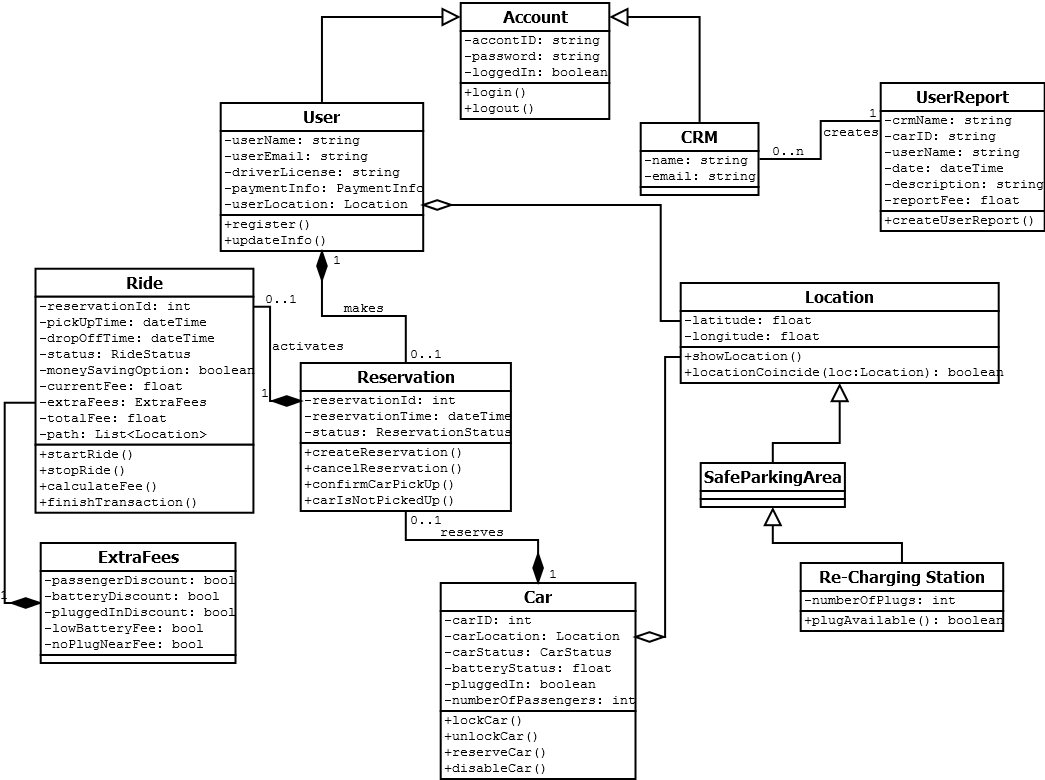
\includegraphics[width=1.27\textwidth]{ClassDiagram.png}}
\caption {Class Diagram}
\vspace*{0.5cm}
\end{figure}
\newpage

\subsection{Sequence Diagrams}
\begin{figure}[h]
\centering
\vspace*{\fill}
\noindent\makebox[\textwidth]{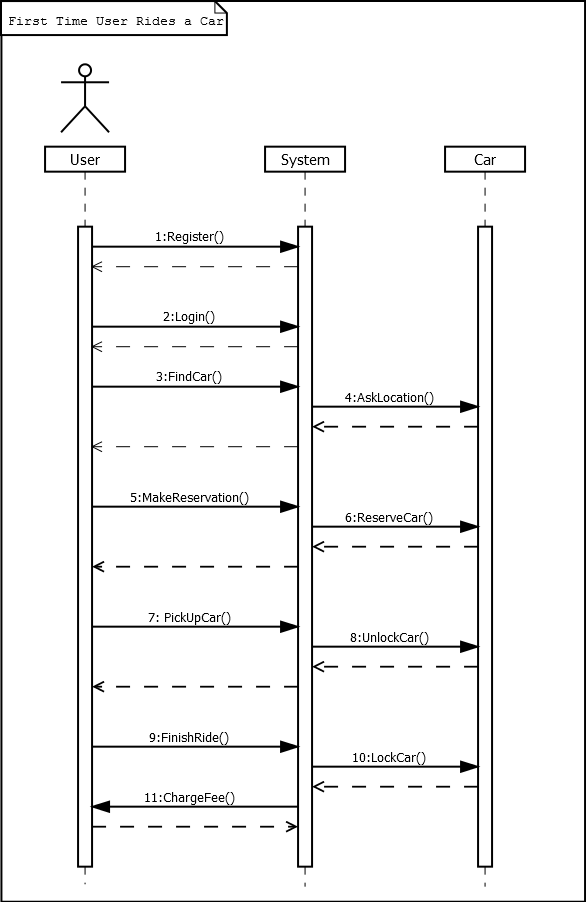
\includegraphics[width = 0.8\textwidth]{SequenceDiagram1.png}}%
\caption {Sequence Diagram 1: User takes a Ride}
\vspace*{0.5cm}
\end{figure}
In the first Sequence Diagram (fig. 3) we abstract the elements present inside the System and show the flow of interaction with the external classes of the System, that is showing the System as a mean to interface the User and the Car. This is presented in a normal case of User asking for a Ride.
\newpage

\begin{figure}[h]
\centering
\vspace*{\fill}
\noindent\makebox[\textwidth]{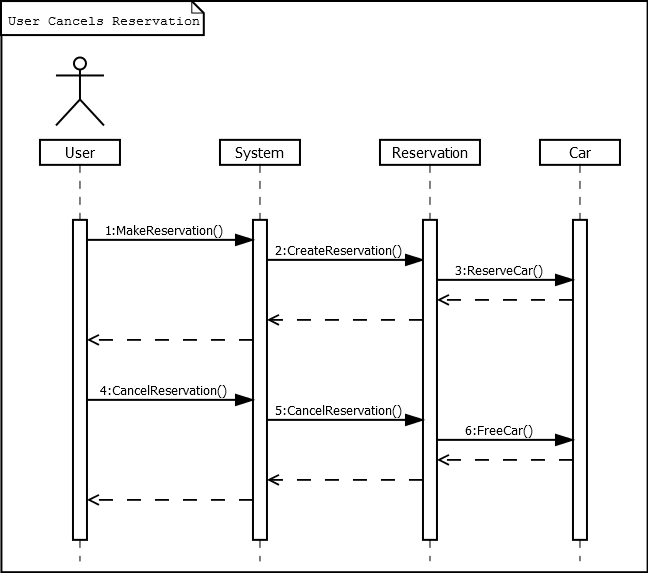
\includegraphics[width=1.2\textwidth]{SequenceDiagram2.png}}%
\caption {Sequence Diagram 2: User cancels a Reservation}
\vspace*{0.5cm}
\end{figure}
In this Sequence Diagram (fig. 4) we represent a sequence within the lifecycle of a Reservation, that is a class which funcionality exists inside the System and serves as the mean for the System to communicate with the Car.
\newpage

\begin{figure}[h]
\centering
\vspace*{\fill}
\noindent\makebox[\textwidth]{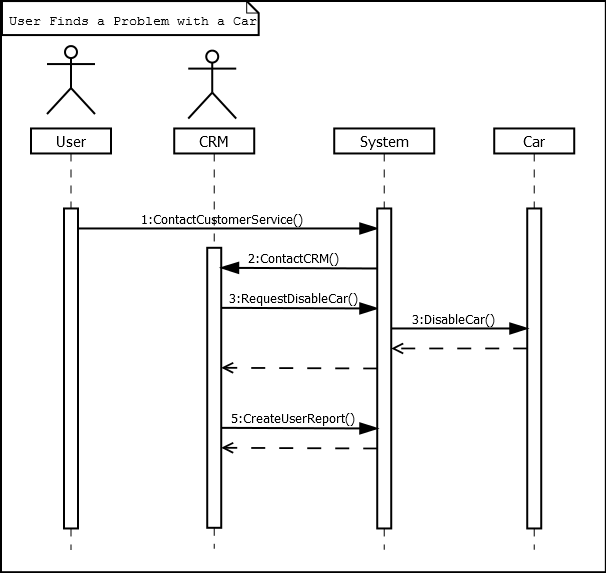
\includegraphics[width=1\textwidth]{SequenceDiagram3.png}}%
\caption {Sequence Diagram 3: User finds a problem with a Car}
\vspace*{0.5cm}
\end{figure}
In this last example of Sequence Diagram (fig. 5) we present a situation in which the User uses the System to interface with our other Actor, the CRM, which in turn uses the System again to interface with the Car.
\newpage

\subsection{Statechart Diagram}
\begin {itemize}
\item \textbf{Reservation:}
\begin{figure}[h]
\centering
\vspace*{\fill}
\noindent\makebox[\textwidth]{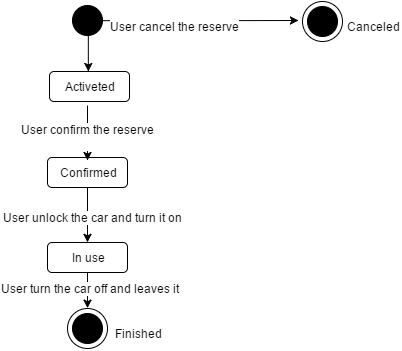
\includegraphics[width=0.7\textwidth]{Reserve.png}}%
\caption {Statechart diagram for the reserve.}
\vspace*{0.2cm}
\end{figure}

\item \textbf{Car:}
\begin{figure}[h!]
\centering
\vspace*{\fill}
\noindent\makebox[\textwidth]{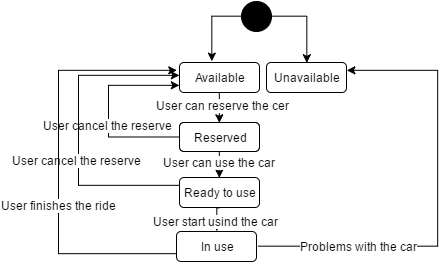
\includegraphics[width=0.8\textwidth]{Car.png}}%
\caption {Statechart diagram for the Car.}
\vspace*{0.2cm}
\end{figure}

\end{itemize}
\newpage

\subsection{Activity Diagram}
\begin{figure}[h]
\centering
\vspace*{\fill}
\noindent\makebox[\textwidth]{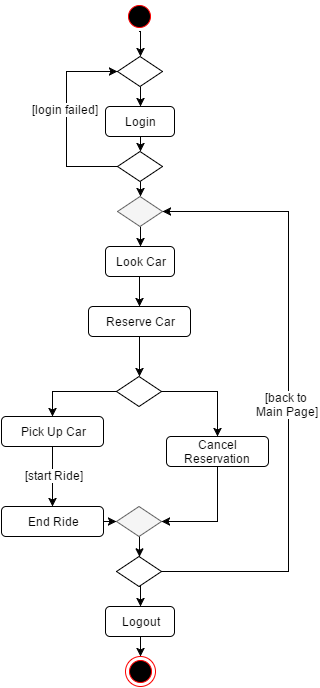
\includegraphics[width=0.59\textwidth]{ActivityDiagram.png}}
\caption {Activity Diagram}
\vspace*{0.1cm}
\end{figure}
\newpage

\section{Alloy Modeling}
\subsection{Model}
The whole system model was implemented in Alloy and the functionalities of  "Login creation" and "Making a new reservation" were tested by the Alloy Analysing tool. These specific functionalities were choosen to be implemented in a formal language for being the key points of the system. 
\subsubsection{Signatures}

\ttfamily
sig Date\{\} \newline
\newline
sig PayInfo\{\} \newline
\newline
sig Location\{ \newline
\hspace*{5 mm}	latitude: Int, \newline
\hspace*{5 mm}	longitude: Int \newline
\} \newline

sig System\{ \newline
\hspace*{5 mm}	listOfRentedCars: set Car, // all reserved cars   \newline
\hspace*{5 mm}	listOfAvailableCars: set Car, // cars that are available for pick up  \newline
\hspace*{5 mm}	listOfReservs: set Reservation, // all active reservations  \newline
\hspace*{5 mm}	listOfAccounts: set Account, // accounts createad  \newline
\hspace*{5 mm}	listofInvoice: set Ride, // Archive of old rides and reservations  \newline
\hspace*{5 mm}	listOfReports: set UserReport //CRM operations  \newline
\} \newline

// User will be considered as a first time user, so it has no attibutes  \newline
sig User\{\} \newline

sig Account\{  \newline
\hspace*{5 mm}	id: one Int, \newline
\hspace*{5 mm}	credentials: one User,  \newline
\hspace*{5 mm}	bankData: one PayInfo, \newline
\hspace*{5 mm}	password: one Int \newline
\} \newline

sig Reservation\{ \newline
\hspace*{5 mm}	id: one Int, \newline
\hspace*{5 mm}	madeBy: one Account, \newline
\hspace*{5 mm}	selectedCar: one Car, \newline
\hspace*{5 mm}	time: one Date, // charging for not picking up the car \newline
\} \newline

sig Car\{ \newline
\hspace*{5 mm}	id: one Int, \newline
\hspace*{5 mm}	loc: one Location, \newline
\hspace*{5 mm}	numOfPassengers: one Int, \newline
\hspace*{5 mm}	battery: one Int, \newline
\}\{ \newline
\hspace*{5 mm}	numOfPassengers < 5 \newline
\hspace*{5 mm}	battery <= 100 \newline
\hspace*{5 mm}	battery >= 0 \newline
\} \newline

sig Ride\{ \newline
\hspace*{5 mm}	reservInQuestion : one Reservation, \newline
\hspace*{5 mm}	timeofPickUp: lone Date, \newline
\hspace*{5 mm}	timeofDropOff: lone Date,  \newline
\hspace*{5 mm}	NotPickUp: one Int, //will be charged fee for not picking up the car \newline
\hspace*{5 mm}	PassengerDisc: one Int, \newline
\hspace*{5 mm}	batteryDisc: one Int, \newline
\hspace*{5 mm}	ReChargingStationDisc: one Int, \newline
\hspace*{5 mm}	HarshConditionsFee: one Int // more then 3km or less the 20\% battery  \newline 
\} \newline

sig SafeParkingArea\{ \newline
\hspace*{5 mm}	zone: set Location  \newline
\} \newline
 
sig ReChargingStation extends SafeParkingArea\{ \newline
\hspace*{5 mm}	spots: set Location -> one Int, //this Int is the number of available plugs \newline
\} \newline

sig Crm\{ \newline
\hspace*{5 mm}	name: String, \newline
\hspace*{5 mm}	email: String \newline
\} \newline

sig UserReport\{ \newline
\hspace*{5 mm}	crmName: Crm, \newline
\hspace*{5 mm}	car: Car, \newline
\hspace*{5 mm}	userName: Account, \newline
\hspace*{5 mm}	reportFee: Int \newline
\} \newline

\rmfamily
\subsubsection{Facts}
 
\ttfamily
//every car, reservation and account is managed by the system \newline
fact systemManagesAll\{ \newline
\hspace*{5 mm}	all c:Car | one s: System | c in (s.listOfRentedCars + s.listOfAvailableCars) \newline
\hspace*{5 mm}	all r:Reservation | one s: System | r in s.listOfReservs \newline
\hspace*{5 mm}	all a:Account | one s:System | a in s.listOfAccounts \newline
\} \newline

fact noCarIntwoLists\{ \newline 
\hspace*{5 mm}	all s:System | \newline
\hspace*{5 mm}	s.listOfRentedCars \& s.listOfAvailableCars = none \newline
\} \newline

fact noFareIn2List\{ \newline
\hspace*{5 mm}	all s:System | \newline 
\hspace*{5 mm}	s.listOfReservs \& s.listofInvoice.reservInQuestion = none \newline	
\} \newline

fact OneFareOneRide\{\newline
\hspace*{5 mm}	no disj f1,f2:Ride, r:Reservation |  f1.reservInQuestion=r and  f2.reservInQuestion=r \newline
\} \newline

fact noDuplicateId\{ \newline
\hspace*{5 mm}	no disj a1, a2: Account | a1.id = a2.id \newline
\hspace*{5 mm}	no disj r1, r2: Reservation | r1.id = r2.id \newline
\hspace*{5 mm}	no disj c1, c2: Car | c1.id = c2.id \newline
\} \newline

\rmfamily
\subsubsection{Login Creation}

\ttfamily
// the same user cannot create two accounts  \newline
fact noUserHas2Accounts\{  \newline 
\hspace*{5 mm}	no disj a1, a2:Account, u: User | a1 != a2 and a1.credentials = u \hspace*{5 mm} and a2.credentials = u  \newline
\}  \newline

// returns a list of accounts that has "a" in it. will be used to assure no duplicates  \newline
fun lookup [a: Account, s: System] : set Account \{  \newline
\hspace*{5 mm}	a \& s.listOfAccounts // \& = intersection  \newline
\} \newline

// the list cannot have more then one item  \newline
fact noDuplicateUser\{  \newline
\hspace*{5 mm}	all a: Account, s:System |  \newline
\hspace*{5 mm}	\#lookup[a, s] < 2  \newline
\}  \newline

// Creating a new account  \newline
pred addAccountToSystem(a:Account, s, s':System)\{  \newline
\hspace*{5 mm}	(s'.listOfAccounts = s.listOfAccounts + a)  \newline
\}  \newline
run addAccountToSystem  \newline

// if two accounts have the same data, they are equal  \newline  
assert addEqualAccount\{  \newline
\hspace*{5 mm}	all a, a':Account, s, s':System |  \newline
\hspace*{5 mm}		addAccountToSystem[a,s,s'] and lookup[a, s'] = lookup[a', s']  \newline
\hspace*{5 mm}		implies  \newline
\hspace*{5 mm}		a = a'   \newline		
\}  \newline
check addEqualAccount for 4 but 1 System  \newline

\rmfamily
\subsubsection{Making a new Reservation}
\ttfamily
fact carOnlyInOneReserv\{ \newline
\hspace*{5 mm}	all c:Car | no disj r1, r2: Reservation | \newline
\hspace*{5 mm}		r1.selectedCar = c and r2.selectedCar = c \newline
\} \newline

fact UserOnlyInOneReserv\{ \newline
\hspace*{5 mm}	all a:Account | no disj r1, r2: Reservation | \newline
\hspace*{5 mm}		r1.madeBy = a and r2.madeBy = a \newline
\} \newline

fact noReservedCars\{ \newline
\hspace*{5 mm}	all c:Car, s:System | \newline
\hspace*{5 mm}	c in s.listOfReservs.selectedCar \newline
\hspace*{5 mm}	implies \newline
\hspace*{5 mm}	c in s.listOfRentedCars \newline
\} \newline

fact noReservedCars2\{ \newline
\hspace*{5 mm}	all c:Car, s:System | \newline
\hspace*{5 mm}	c not in s.listOfReservs.selectedCar \newline
\hspace*{5 mm}	implies \newline
\hspace*{5 mm}	c in s.listOfAvailableCars \newline
\} \newline

pred createReservation[a: Account, c:Car, r,r': Reservation]\{ \newline
\hspace*{5 mm}		r'.id = r.id + 1 \newline
\hspace*{5 mm}		r'.madeBy = a \newline 
\hspace*{5 mm}		r'.selectedCar = c \newline 
\hspace*{5 mm}		r'.time = Date \newline
\} \newline
run createReservation \newline

pred makeReservation[a: Account, c:Car, s,s',s'': System, r, r':Reservation]\{ \newline
\hspace*{5 mm}		// create a reservation \newline
\hspace*{5 mm}		createReservation[a, c, r,r']  \newline
\hspace*{5 mm}		// add reservation the the list \newline	
\hspace*{5 mm}		s'.listOfReservs = s.listOfReservs + r' \newline
\hspace*{5 mm}		// change car list  \newline
\hspace*{5 mm}		s'.listOfAvailableCars = s.listOfAvailableCars - c \newline
\hspace*{5 mm}		s''.listOfRentedCars = s'.listOfRentedCars + c \newline
\} \newline
run makeReservation for 5 but 3 Reservation, 1 System  \newline

assert sameCar2Reserv\{ \newline
\hspace*{5 mm}		no disj a1,a2:Account, s1,s2,s3:System, c:Car, r1,r2, r3:Reservation | \newline
\hspace*{5 mm}			makeReservation[a1, c, s1,s2,s3, r1,r2] and makeReservation[a2, c, s1,s2,s3, r2,r3] \newline
\} \newline
check sameCar2Reserv \newline

assert sameUser2Reserv\{ \newline
\hspace*{5 mm}		no disj c1,c2:Car, a:Account, s1,s2,s3:System, r1,r2, r3:Reservation| \newline
\hspace*{5 mm}			makeReservation[a, c1, s1,s2,s3, r1,r2] and makeReservation[a, c2, \hspace*{5 mm}	s1,s2,s3, r2,r3] \newline
\} \newline
check sameUser2Reserv \newline
\rmfamily

\subsection{Alloy Result}
As stated  in the previous Alloy code, the following checks were made:
\begin{itemize}
\item Adding an account to the system
\item Trying to add two equal accounts
\item Creating a new reservation
\item Creating a new reservation and integrating it with the rest of the system
\item Trying to reserve the same car twice
\item The same user tries to make two reservations
\end{itemize}

The Alloy Analyser tool gave the following feedback:

\begin{figure}[h]
\centering
\vspace*{\fill}
\noindent\makebox[\textwidth]{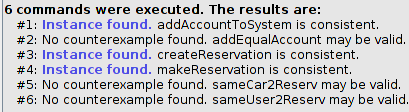
\includegraphics[width = 0.8\textwidth]{tests.png}}%
\caption {Alloy result}
\vspace*{0.5cm}
\end{figure}
This result proves our model is mathematically consistent for the implemented cases.

\subsection{Generated World}
Each of the worlds generated with the Alloy Analysing tool are consistent with the proposed system. Special attention was given for the relations between entities to respect especific rules that could potentially cause inconsistency in the system with its use, as not allowing duplicates or always making sure that cars that appears in reservations are placed only in the rented cars list.   

\begin{figure}[h]
\centering
\vspace*{\fill}
\noindent\makebox[\textwidth]{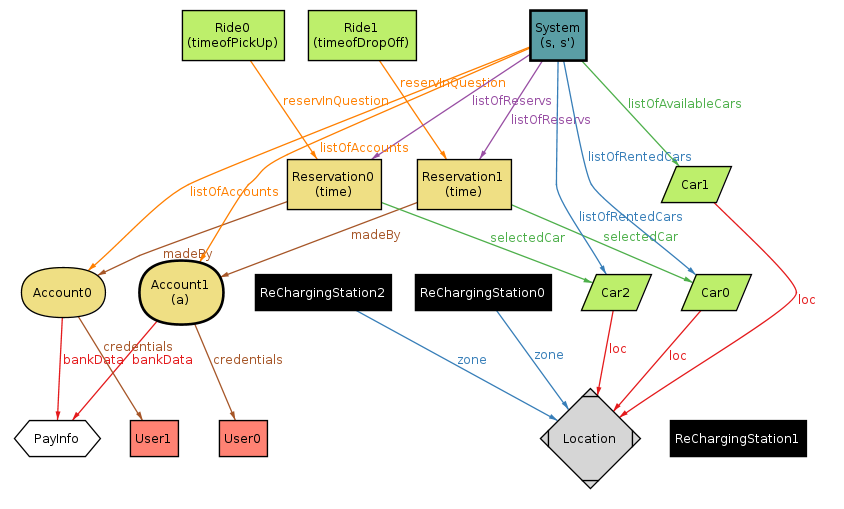
\includegraphics[width = 1.3\textwidth]{world1.png}}%
\caption {First generated instance}
\vspace*{0.5cm}
\end{figure}

\begin{figure}[h]
\centering
\vspace*{\fill}
\noindent\makebox[\textwidth]{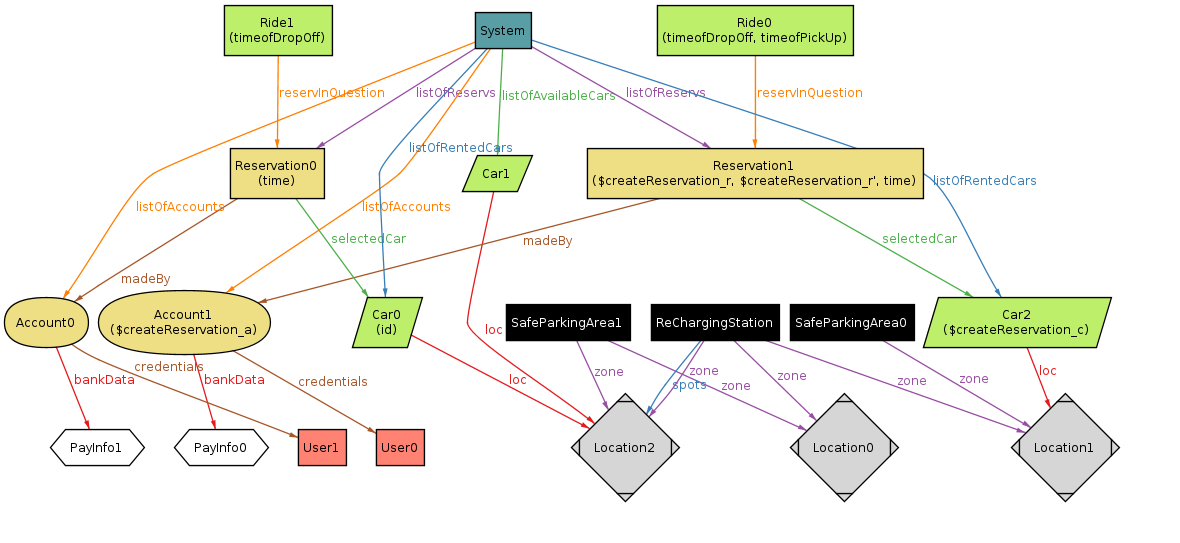
\includegraphics[width = 1.5\textwidth]{world2.png}}%
\caption {Second generated instance}
\vspace*{0.5cm}
\end{figure}

\begin{figure}[h]
\centering
\vspace*{\fill}
\noindent\makebox[\textwidth]{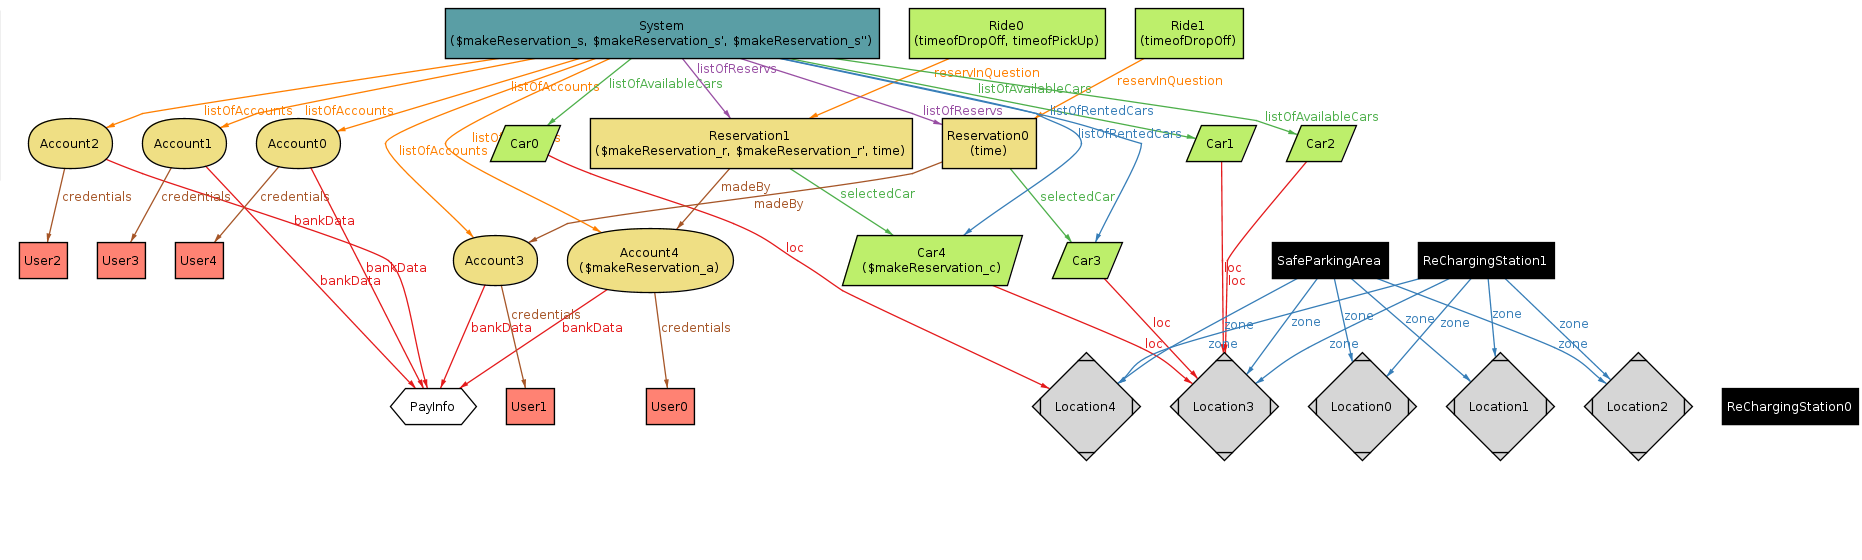
\includegraphics[width = 1.7\textwidth, angle =90]{world3.png}}%
\caption {Third generated instance}
\vspace*{0.5cm}
\end{figure}

\section{Used Tools}
The Tools used to develop this RASD document were:
\begin{itemize}
	\item \textbf{GitHub:} for Version Control
	\item \textbf {Dia Diagram Editor:} for UML Diagrams
	\item \textbf{Alloy Analyzer 4.2:} for Alloy Modelling and proving consistency
	\item \textbf {TeXworks:} for LaTex editing of this Document
	\item \textbf {Microsoft PowerPoint:} for Proposed System and Presentation
	\item \textbf {Draw.io:} for Activity and Statechart Diagrams
	\item \textbf {Balsamiq Mockups 3:} for UI Screen Mockups
\end{itemize}
\newpage

\section{Hours of Work}
\begin{tabular}{ | l | l | l | l | }
\hline
	\textbf {Date} & \textbf {Domenico} & \textbf {Caio} & \textbf {Matheus} \\ \hline
	25/10/16& 30m & 30m & 30m \\ \hline
	26/10/16& 1h & -  & -  \\ \hline
	27/10/16&  - & - & -  \\ \hline
	28/10/16& 2h.30m & 4h.30m & 4h.30m \\ \hline
	29/10/16& 1h & -  & - \\ \hline
	30/10/16&  1h & - & 2h\\ \hline
	31/10/16&  - & 2h & - \\ \hline
	01/11/16&  - & - & 2h \\ \hline
	02/11/16&  2h & - & - \\ \hline
	03/11/16&  2h & 3h & 3h \\ \hline
	04/11/16&  - & - & 2h\\ \hline
	05/11/16&  2h & 4h &  6h\\ \hline
	06/11/16&  - & 5h & 6h\\ \hline
	07/11/16& 4h & 2h & 6h \\ \hline
	08/11/16&  3h & - & - \\ \hline
	09/11/16&  2h & 2h & 3h \\ \hline
	10/11/16&  3h & 3h & 2h\\ \hline
	11/11/16&  2h & 2h & - \\ \hline
	12/11/16&  3h & 3h & - \\ \hline
\end{tabular}

\newpage

\section{Changelog}
As the project and design decisions may change during the development this document is also prone to change.
We'll document every version in this part.
\begin{itemize}
\item \textbf {Version 1.1:} 12/11/2016
\end{itemize}
\end{document}
